\paragraph{Requirements}
Imaging system: 
\begin{itemize}
    \item Limited to using raspberry Pi 3 B+ as on-board computer due to budget.
    \item The delay of image transfer should be less than 1 second, ignore wireless transfer time. 
    \item Images should be tagged in real time with no delay. 
\end{itemize}
\paragraph{Camera}
%Identify the camera used by UAS and describe its capabilities, provide a detailed analysis to demonstrate that the chosen camera can resolve objects of the size required by the competition.%

The team's budget for camera was approximately \$800 CAD, and most of the high-end research cameras cost more than \$1000 CAD without the lens. The goal is to capture high resolution images to yield a wide ground area coverage per image, all the while staying under the proposed budget. Digital single-lens reflex (DSLR) cameras with their large Complementary metal–oxide–semiconductor (CMOS) sensor fit the team requirements. Refer to Table 4 for all the cameras under consideration.

\begin{figure}[H]\centering
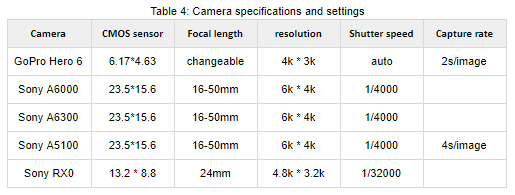
\includegraphics[width=\linewidth]{table/Table_4_camera_specs.PNG}
\caption*{}
\label{fig:cs}
\end{figure}

After taking the size of the camera into consideration, the SONY A5100 is clearly the best choice since although A6000, A6300 and A5100 all have similar image quality, but unlike the rest the the Sony A5100 doesn't use a optical view finder, which greatly reduced it's size,  weight and price. Although it's battery life is not ideal for the long flight time, an external charging port is used to replace the internal battery to overcome that limitation. What's more, Sony A5100 is one of the cameras supported by gphoto2 API, which simplified it's programming interface. 

\paragraph{Gimbal} 
Five different gimbal configurations were considered: using brushless motors or servo motors, with 2 axis, 1 axis or no gimbal at all. The major requirements were the weight and angle of operation. As per flight data, Condor has a maximum forward bank of 35$^{\circ}$, up to 40$^{\circ}$ when flying at 25m/s. Consequently, the 40$^{\circ}$ pitch angle in forward and 15$^{\circ}$ in backward were reserved; images will not be captured when flying backwards. Next, the gimbal control was chosen from three options: use a dedicated controller like BASECAM BGC, create a custom controller from scratch or use Mission planner's gimbal control feature. Optimizing the weight of payload, the team decided to go with the custom option, using a small and light weight servo motor. The chosen camera, Sony A5100, has a length x height of 110 x 63mm. To allow the gimbal to enclose this large camera and still function properly, the decision to use a single axis gimbal was made. This axis is being used to stabilize the large angle forward pitch. Any small roll angles will be accounted for through the software calibrating the images. 

\paragraph{Image transfer software}
During flight, images are taken by the UAV and geotagged with relevant flight data — latitude, longitude, altitude, heading, roll—using the DroneKit-Python SDK (Software Development Kit). Images are then live-transferred from the onboard Raspberry Pi to the GCOMv2 (Ground Command version 2), UBC UAS’ ground control software suite—server using Lsyncd—Live syncing daemon, a tool used for local and remote directory synchronization. Lsyncd monitors for file events on the Pi and aggregates and combines these events, spawning an rsync/SSH (Secure Shell) process to replicate these changes to the GCOMv2 server. To minimize bandwidth consumption, Lsyncd is configured to compress and uncompress the payload sent. For extra security, communication between the Pi and the server is authenticated using RSA (Rivest–Shamir–Adleman) encrypted private-public keys. 

The imaging transferring stack has been thoroughly tested by configuring a near identical system, consisting of two servers and a simulated live image capturing stream. Image transferring speed and stability are ensured with the help of Lsyncd’s compression transferring and a stable network connection. To maximize reliability, a custom script is run on the Pi to automatically reboot Lsyncd in the case of a system malfunction, such as a disconnection.
